\chapter{Theoretical background}
\label{chap:refs}

\section{Glossary}

\paragraph{SDN} Software-defined network. Additional details can be found in \xxx{\cref{TODO}}.

\paragraph{OVS} Open vSwitch\footnote{\url{https://www.openvswitch.org/}}

\paragraph{OVN} Open Virtual Network\footnote{\url{https://docs.ovn.org/en/latest/}}

\paragraph{CNI} Container network interface\footnote{\url{https://github.com/containernetworking/cni/blob/dc0779e8cec8bfe39bc0d7a038250e233e5214eb/SPEC.md}}. Specification for writing plugins configuring network interfaces in Linux container, best known by usage in Kubernetes.

\paragraph{OVN-Kubernetes} CNI plugin using OVN.

\paragraph{Forwarding table} Network switches use forwarding tables to decide where to forward a received packet. In Ethernet, the forwarding tables consist of MAC address to network port mapping. SDNs generalized forwarding tables so that they can match packets in any way deemed useful, most commonly on any header values from the second, third, and fourth layers of the OSI model.\todo{quote \url{https://www.iso.org/standard/20269.html}}

\paragraph{OpenFlow} Network configuration protocol used between an SDN controller and SDN switches. OpenFlow allows remote configuration of forwarding tables in network switches.


\section{Software-defined networking (SDN)}
\todo{make a proper quotation for the schema in \cref{fig:sdn-schema} \url{https://opennetworking.org/wp-content/uploads/2013/02/TR_SDN_ARCH_1.0_06062014.pdf}}

\begin{figure}
    \centering
    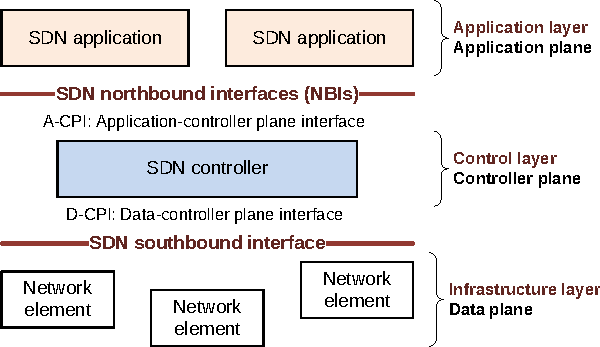
\includegraphics[width=.6\linewidth]{img/sdn_basic_schema.pdf}
    \caption{A schema of basic SDN components.}
    \label{fig:sdn-schema}
\end{figure}

\emph{Software-defined networking} is a loosely defined concept of separating the networking data plane (infrastructure layer) and the control plane (control layer) into separate components. In traditional networking architectures, each network device makes forwarding and/or routing decisions fully autonomously. SDNs separate the decision-making and data processing into distinct layers (see \cref{fig:sdn-schema}) and define two main interfaces. \emph{SDN applications} provide the \emph{SDN controller} with networking requirements using the \emph{northbound interface}. The controller then configures the actual network equipment using the \emph{southbound interface}.

\emph{OpenFlow}\footnote{\url{https://opennetworking.org/sdn-resources/openflow-switch-specification/}} is a de-facto standard protocol for the southbound interface. \emph{Container network interface (CNI)} is a specification for the northbound interface in Kubernetes and other container orchestrators.

\section{OpenFlow}

\todo{add a proper example to the table}

\emph{OpenFlow} is a protocol for configuring packet forwarders (generalized switches). The forwarding tables (see \cref{tab:openflow-forwarding-table}) in the network switches are filled with rules provided by the OpenFlow controller. The flow rules consist of two parts:

\begin{itemize}
    \item \emph{Packet matching criteria} which can include value masks for not only Ethernet header values, but also IP, transport layer protocols (TCP, UDP, ...), and more depending on the version of the OpenFlow protocol. 
    \item The action instructing the switch on what to do with the matching packets. Possible actions include dropping packets, modifying header fields, forwarding to physical or virtual ports, sending to the controller, and more.
\end{itemize}

In addition to the externally configured flow rules, the forwarding tables also contain statistics updated every time the flow rule is used. The OpenFlow controller can then query switches for these statistics.

\begin{table}[]
    \begin{center}
        \caption{Schema of an OpenFlow forwarding table}
        \label{tab:openflow-forwarding-table}
        \begin{tabular}{c|c|c}
            \textbf{Matching criteria} & \textbf{Action} & \textbf{Statistics} \\
            \hline
            \xxx{add example} & 1110.1 & a\\ % <--
            2 & 10.1 & b\\ % <--
            3 & 23.113231 & c\\ % <--
        \end{tabular}
    \end{center}
\end{table}


\section{Open vSwitch}

\emph{Open vSwitch} (OVS) is a multilayer virtual switch. OVS runs as a software switch on all major platforms and supports hardware offload for its data processing layers. The supported OpenFlow protocol allows any SDNs to use OVS in its infrastructure layer.

The internal architecture of OVS mirrors the SDN architecture (see \cref{fig:ovs-arch-schema}\todo{redraw the image or quote it properly}). \ident{ovs-vswitchd} (or just \ident{vswitchd}) is the OVS's control process. \ident{vswitchd} communicates via the OpenFlow protocol and stores the configured flow rules in a purpose-built Open vSwitch Database (OVSDB). Alternatively, the database can be accessed externally, and OVS can be configured without using the OpenFlow wire protocol.

A \emph{datapath} is the lowest component of OVS physically forwarding packets between configured ports. There are multiple datapath implementations, some of them implemented fully in the \ident{vswitchd} process, some of them using extra kernel modules for improved performance. \ident{vswitchd} translates the OpenFlow flow rules into a more efficient and simplified form. These simplified flow rules are then used by the datapaths to make forwarding decisions.

\begin{table}[h!]
    \begin{center}
        \caption{Overview of OVS components}
        \label{tab:ovs-components}
        \begin{tabular}{p{0.2\linewidth}|p{0.7\linewidth}}
            \textbf{Component} & \textbf{Description} \\
            \hline
            % FIXME this footnote might be on a wrong page :(
            \ident{ovsdb}\tablefootnote{\url{https://docs.openvswitch.org/en/latest/ref/ovsdb.7/}} & OVSDB instance storing the OpenFlow flow rules \\
            \hline
            \ident{ovs-vswitchd}\tablefootnote{\url{http://www.openvswitch.org/support/dist-docs/ovs-vswitchd.8.html}} & a process managing datapaths and providing OpenFlow configuration interface \\
            \hline
            datapath & a logical component in \ident{ovs-vswitchd}, does the actual packet forwarding \\
        \end{tabular}
    \end{center}
\end{table}


\section{Open Virtual Network}

\todo{link to documentation \url{https://access.redhat.com/documentation/en-us/red_hat_openstack_platform/13/html/networking_with_open_virtual_network/open_virtual_network_ovn}}

\emph{Open Virtual Network} (OVN) is an SDN combining Open vSwitch with network tunnels (by default GENEVE) for its infrastructure layer. Applications communicate with OVN through the \ident{northdb}, an OVSDB instance storing high-level network configuration in terms of traditional networking concepts. The \ident{ovn-northd} process translates the configuration into logical datapath flows and stores the result in the \ident{southdb} OVSDB instance. The \ident{ovn-controller} then distributes the flows from the \ident{southdb} into individual OVS databases.

\begin{table}[h!]
    \begin{center}
        \caption{Overview of OVN components}
        \label{tab:ovn-components}
        \begin{tabular}{p{0.23\linewidth}|p{0.47\linewidth}|p{0.2\linewidth}}
            \textbf{Component} & \textbf{Description} & \textbf{How it runs} \\
            \hline
            \ident{northdb} & OVSDB instance storing network configuration in terms of traditional networking concepts & centralized or distributed \\
            \hline
            \ident{ovn-northd} & process translating configuration into logical flows & centralized or distributed \\
            \hline
            \ident{southdb} & OVSDB instance storing network configuration in terms of logical flows & centralized or distributed\\
            \hline
            \ident{ovn-controller} & configures local OVS from the \ident{southdb} & locally on every node\\
        \end{tabular}
    \end{center}
\end{table}


\section{OVN-Kubernetes}

\emph{OVN-Kubernetes}\footnote{\url{https://github.com/ovn-org/ovn-kubernetes}} is a Kubernetes CNI plugin using OVN in the background. \todo{Expand with information about internal architecture.}

\section{Open vSwitch Datapath Internals}
\label{sec:ovs-internals}
\todo{This whole section is not adapted to the thesis yet. It is just copy-pasted from my website.}

\begin{figure}
    \centering
    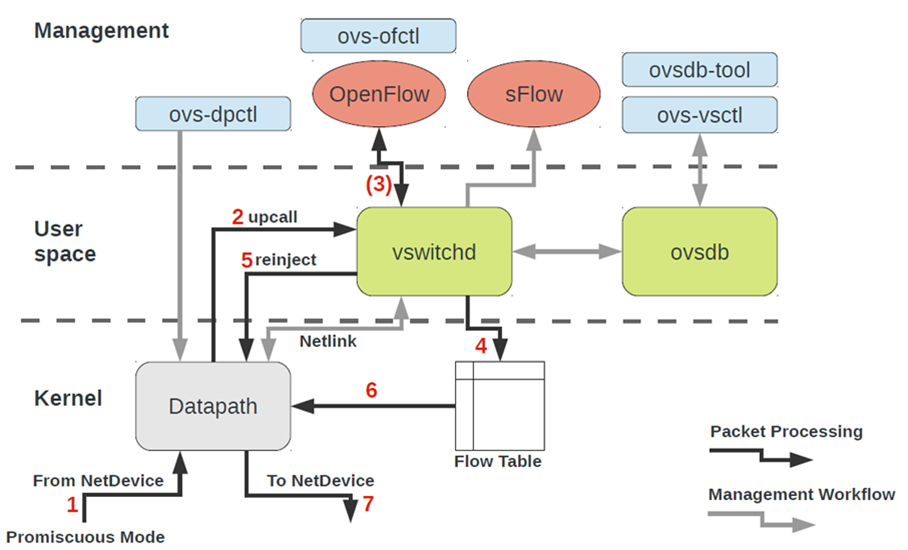
\includegraphics[width=.9\linewidth]{img/ovs_architecture_01.png}
    \caption{Schema of OVS internal architecture.}
    \label{fig:ovs-arch-schema}
\end{figure}

\ident{ovs-vswitchd} processes packets in \href{https://github.com/openvswitch/ovs/blob/e90a0727f17f6ad915a32735a8c0b282f2c8cd6f/lib/dpif.h}{datapaths}, which is essentially \href{https://github.com/openvswitch/ovs/blob/e90a0727f17f6ad915a32735a8c0b282f2c8cd6f/lib/dpif-provider.h\#L107-L117}{an interface} hiding the implementation details of low-level packet processing. The datapath does not do any decisions by itself, it's the clients of the datapath that tell it what to do by giving it simple rules to follow. In the upstream code, there are two datapath implementations - \href{https://github.com/openvswitch/ovs/blob/e90a0727f17f6ad915a32735a8c0b282f2c8cd6f/lib/dpif-netdev.c}{\ident{netdev}} and \href{https://github.com/openvswitch/ovs/blob/e90a0727f17f6ad915a32735a8c0b282f2c8cd6f/lib/dpif-netlink.c}{\ident{netlink}}.

The \ident{netdev} datapath is implemented entirely in user space, and it's multiplatform. All major operating systems are currently supported. As it's userspace only, it's less performant than the \ident{netlink} datapath and we will ignore it for the rest of this article. The \ident{netlink} datapath is Linux-specific. It resides partially in a kernel module and partially in user space. The kernel module does most of the packet processing. The userspace communicates with the kernel over a netlink socket, exchanging commands and packets. Most packets never touch the user space and are processed only in the kernel. We call this the fast-path. The alternative is the slow-path, a path through user space, which is taken every time the fast-path fails.


\subsection{Overview of the kernel and user space interactions}
\label{overview-of-the-kernel-and-user-space-interactions}

The fast-path involves matching incoming packet against a set of flow rules stored in the kernel. The rules contain actions -- instructions describing what to do next with the packet. If any of the flow rules matches, the kernel blindly executes the action. In this case, no buffering is involved, the packets are processed immediately.

The slow-path gets involved when the fast-path fails (no flow rule match) or when the action in the flow rule asks for it. In it, the packet is passed to the user-space via a netlink socket (we call this an upcall). An user-space process receives the packet, processes it according to its configuration and reinjects it back into the kernel. Additionally, a new flow rule can be installed into the kernel to speed up future processing of similar packets. The slow-path buffers packets when they are passed from kernel to user-space.

\subsection{The fast-path}
\label{the-fast-path}

\subsubsection{The data structures}
\label{the-data-structures}

The flow table (\href{https://elixir.bootlin.com/linux/v6.2.6/source/net/openvswitch/flow_table.h\#L62}{\ident{struct\ flow\_table}}) is an in-kernel data structure, which stores flows rules (\href{https://elixir.bootlin.com/linux/v6.2.6/source/net/openvswitch/flow.h\#L221}{\ident{struct\ sw\_flow}}) and allows for fast matching with individual packets. Every flow also contains a list of actions (\href{https://elixir.bootlin.com/linux/v6.2.6/source/net/openvswitch/flow.h\#L206}{\ident{struct\ sw\_flow\_actions}}).

Every flow has a flow key (\href{https://elixir.bootlin.com/linux/v6.2.6/source/net/openvswitch/flow.h\#L75}{\ident{struct\ sw\_flow\_key}}) and a bitmask (\href{https://elixir.bootlin.com/linux/v6.2.6/source/net/openvswitch/flow.h\#L183}{\ident{struct\ sw\_flow\_mask}}). The combination of both of these enables the packet matching. The key is a complex structure with parsed out packet header values. It can be created from any Ethernet frame (\href{https://elixir.bootlin.com/linux/v6.2.6/source/net/openvswitch/flow.c\#L886}{\ident{key\_extract}}). The mask then tells us which bits between the extracted packet key and the flow key must match.


\subsubsection{The matching algorithm}
\label{the-matching-algorithm}

When processing a packet, we create the corresponding flow key and look for matching flows in the flow table. The packet can match any number of flows, but we always use the first one we find. The userspace component is made responsible for preventing overlapping conflicting flow rules.

The flow table stores the flow in a hash table, where the key is the masked \ident{sw\_flow\_key}. Therefore, to find a flow for a packet, we must try several masks. The lookup procedure could look like this:

\begin{verbatim}
    def lookup(flow_table, key):
        for mask in flow_table.mask_array:
            masked_key = apply mask to key
            if masked_key in flow_table.flows:
                return flow_table.flows[masked_key]
        return None
\end{verbatim}
    

The real implementation (\href{https://elixir.bootlin.com/linux/v6.2.5/source/net/openvswitch/flow_table.c\#L785}{\ident{ovs\_flow\_tbl\_lookup\_stats}}) is in principle similar, but more optimized:

\begin{enumerate}
\def\labelenumi{\arabic{enumi}.}
\item
  The kernel keeps mask usage statistics and the \ident{mask\_array} is
  kept sorted with the most used masks first
  (\href{https://elixir.bootlin.com/linux/v6.2.5/source/net/openvswitch/flow_table.c\#L1107}{\ident{ovs\_flow\_masks\_rebalance}}).
  This happens
  \href{https://elixir.bootlin.com/linux/v6.2.5/source/net/openvswitch/datapath.c\#L2536}{periodically}
  based on a time interval.
\item
  There is already a \ident{sk\_buff}
  \href{https://elixir.bootlin.com/linux/v6.2.5/source/include/linux/skbuff.h\#L1537}{hash}
  based on source/destination addresses and ports. The lookup procedure
  makes use of the hash by having a fixed size
  (\href{https://elixir.bootlin.com/linux/v6.2.5/source/net/openvswitch/flow_table.c\#L41}{256})
  hash table storing references to their masks. The cached masks are
  then tried first. If there is no match, standard lookup over all masks
  follows. This helps with burst performance.
\end{enumerate}

\subsection{The slow-path}
\label{the-slow-path}

The user space process (\href{https://www.man7.org/linux/man-pages/man8/ovs-vswitchd.8.html}{\ident{ovs-vswitchd}}) communicates with the kernel over netlink socket. When packet leaves the
fast-path, it is temporarily buffered in a queue (\href{https://elixir.bootlin.com/linux/v6.2.6/source/net/openvswitch/datapath.c\#L311}{\ident{ovs\_dp\_upcall}}) when crossing the kernel boundary.

\ident{ovs-vswitchd} reads packets from the kernel in several threads. The datapath interface defines a \href{https://github.com/openvswitch/ovs/blob/e90a0727f17f6ad915a32735a8c0b282f2c8cd6f/lib/dpif-provider.h\#L387-L408}{\ident{recv}} function for receiving a single packet from the kernel. The netlink datapath implements it with the function \href{https://github.com/openvswitch/ovs/blob/e90a0727f17f6ad915a32735a8c0b282f2c8cd6f/lib/dpif-netlink.c\#L3132-L3134}{\ident{dpif\_netlink\_recv}}.

Higher up, the \ident{recv} datapath interface function is used in generic \href{https://github.com/openvswitch/ovs/blob/e90a0727f17f6ad915a32735a8c0b282f2c8cd6f/lib/dpif.c\#L1591-L1611}{\ident{dpif\_recv}} which also provides an useful tracepoint \href{https://github.com/openvswitch/ovs/blob/e90a0727f17f6ad915a32735a8c0b282f2c8cd6f/lib/dpif.c\#L1618}{\ident{dpif\_recv\_\_recv\_upcall}} for measurements. Even higher up the abstraction stack, the function \href{https://github.com/openvswitch/ovs/blob/e90a0727f17f6ad915a32735a8c0b282f2c8cd6f/ofproto/ofproto-dpif-upcall.c\#L829-L830}{\ident{recv\_upcalls}} in the file \ident{ofproto-dpif-upcall.c} reads packets in batches, which are then processed by \href{https://github.com/openvswitch/ovs/blob/e90a0727f17f6ad915a32735a8c0b282f2c8cd6f/ofproto/ofproto-dpif-upcall.c\#L1639-L1641}{\ident{handle\_upcalls}}. The \ident{handle\_upcalls} function essentially transforms the list of packets into a list of operations that should be executed on the datapath. This includes adding new flows to the datapath as well as simply sending packets where they belong.

Parallel with upcall processing, OVS also runs several maintenance tasks. A \href{https://github.com/openvswitch/ovs/blob/e90a0727f17f6ad915a32735a8c0b282f2c8cd6f/ofproto/ofproto-dpif-upcall.c\#L3312-L3336}{balancing task} makes sure, that when the system is under stress, the most used flow rules are in the kernel. \href{https://github.com/openvswitch/ovs/blob/e90a0727f17f6ad915a32735a8c0b282f2c8cd6f/ofproto/ofproto-dpif-upcall.c\#L83-L111}{A revalidator task} periodically reads statistics from the kernel and most importantly, removes old unused flows.

% TODO add sources
%
% \begin{center}\rule{0.5\linewidth}{0.5pt}\end{center}
% 
% \hypertarget{sources}{%
% \section{Sources}\label{sources}}
% 
% \begin{itemize}
% \tightlist
% \item
%   \href{https://docs.openvswitch.org/en/latest/contents/}{Open vSwitch
%   online documentation}
% 
%   \begin{itemize}
%   \tightlist
%   \item
%     \href{https://docs.openvswitch.org/en/latest/topics/datapath/}{Open
%     vSwitch Datapath Development Guide}
%   \end{itemize}
% \item
%   \href{https://elixir.bootlin.com/linux/v6.2.6/source}{Linux Kernel
%   source code}
% \item
%   \href{https://github.com/openvswitch/ovs/tree/51778134d4c8a84801230b1e5a7d59e180d9e8b5}{Open
%   vSwitch source code}
% \item
%   \href{https://developers.redhat.com/articles/2022/02/07/investigating-cost-open-vswitch-upcalls-linux}{RedHat
%   Developer Blog: Investigating the cost of Open vSwitch upcalls in
%   Linux}
% \item
%   \href{https://hustcat.github.io/an-introduction-to-ovs-architecture/}{An
%   introduction to OVS architecture}
% \end{itemize}